\documentclass[a4paper]{article}

\usepackage[width=14cm, left=3cm, top=3cm]{geometry}

\usepackage[brazil]{babel}
\usepackage[T1]{fontenc}
\usepackage[utf8]{inputenc}

\usepackage{hyperref}

\usepackage{graphicx}

\usepackage{amsmath}
\usepackage{amssymb}

% No indent
\setlength{\parindent}{0pt}
\setlength{\parskip}{2ex}

\newcommand{\linkfileraw}[2]{\href{run:../../#1}{\texttt{#2}}}
\newcommand{\linkfile}[2][src/05-finite-elements-gamma/]{\linkfileraw{#1#2}{#2}}

\newcommand{\typ}{:\,}

\newcommand{\vphi}{\varphi}

\title{Trabalho 02 --- Elementos Finitos}
\author{Daniel Kiyoshi Hashimoto Vouzella de Andrade -- 124259224}
\date{?? de Outubro de 2024}

\begin{document}
\maketitle

\setcounter{section}{-1}
\section{Implementação (TODO)}

A implementação (e esse pdf) está em
\href{https://github.com/Kiyoshi364/finite-elements}{github.com/Kiyoshi364/finite-elements}.
O pdf está sendo feio em cima do commit
\texttt{365e28bbdca537e48f6eb6afc77e6756017df39a},
então o commit de entrega deve ser o seguinte a esse.

A implementação está na pasta
\linkfileraw{/src/05-finite-elements-gamma/}{/src/05-finite-elements-gamma/},
(os outros arquivos serão indicados
relativamente a essa pasta).
O arquivo \linkfile{finite-elements.jl}
é ``a biblioteca'',
enquanto
\linkfile{solution.jl} e \linkfile{errors.jl}
são os ``scripts'' que rodam os experimentos pedidos
e geram as imagens incluídas no final do pdf\footnote{
Para que os scripts gerem uma imagem,
é necessário alterar o nome do arquivo de saída
em cada script para ter uma extensão de imagem
(ou não ter extensão nenhuma).
Por padrão eles geram um pdf.
}.
Para que os exemplos que os scripts rodam
sejam o mesmo do pedido
(\(u(x) = \sin(\pi \; x)\)),
escolha o exemplo \(0x3\)
no início dos scripts.
O exemplo está definido
no arquivo
\linkfile{../examples.jl}
na função \texttt{bacarmo\_example\_gamma}.
Outro arquivo usado pela biblioteca é
\linkfile{../common.jl}
que possui algumas funções e códigos auxiliares,
como cálculo de erro e
tabela de pontos e pesos da quadratura de Gauss.

\section{Formulação Forte}

Dados
\(f \typ [0, 1] \times [0, T] \to \mathbb{R}\),
\(u_0 \typ [0, 1] \to \mathbb{R}\),
\(g \typ \mathbb{R} \to \mathbb{R}\),
\(T \ge 1\),
\(\alpha > 0\),
\(\beta \ge 0\),
\(\gamma \ge 0\),
o objetivo é descobrir \(u \typ [0, 1] \times [0, T] \to \mathbb{R}\)
que satisfaça o sistema:
\[ \begin{cases}
    u'(x, t) - \alpha \; u_{xx}(x) + \beta \; u(x) + \gamma \; u_{x}(x) + g(u(x, t))= f(x, t)
        &\quad\text{, } x \in \,]0, 1[ \text{ , } t \in \,]0, T]
    \\
    u(0, t) = u(1, t) = 0
        &\quad\text{, } t \in [0, T]
    \\
    u(x, 0) = u_0(x)
        &\quad\text{, } x \in \,]0, 1[
\end{cases} \]

É conveniente definir
para cada \(u \typ [0, 1] \times [0, T] \to \mathbb{R}\)
para cada \(t \in \,]0, T]\),
uma \(u(t) \typ [0, 1] \to \mathbb{R}\)
tal que
\(
    u(t)(x) = u(x, t)
\).

\section{Transição entre Forte e Fraca}

Sejam o espaço das soluções:
\[
    H = \{
        u \text{ é suficientemente suave } : u(0) = u(1) = 0
    \}
\]
e o espaço das funções de teste (funções peso)
\[
    V = \{
        v \text{ é suficientemente suave } : v(0) = v(1) = 0
    \}
\]

\emph{Nota}: Nesse caso \(H = V\).

Seja \(v \in V\) qualquer,
simplificamos (enfraquecemos)
o termo de \(\alpha\)
do problema inicial:
\[ \begin{array}{l}
    - \alpha \; \int_0^1{ u_{xx}(x, t) \; v(x) \; dx }
    \\[1ex]
    - \alpha \; \left[ \left( v(x) \; u_x(x, t) \right|_0^1 - \int_0^1{ u_x(x, t) \; v_x(x) \; dx } \right]
    \\[1ex]
    - \alpha \; \left[ - \int_0^1{ u_x(x, t) \; v_x(x) \; dx } \right]
    \\[1ex]
    \alpha \; \int_0^1{ u_x(x, t) \; v_x(x, t) \; dx }
\end{array} \]

Juntando tudo:
\[ \begin{cases}
    \int_0^1{ u'(x, t) \; v(x) \; dx}
    + \alpha \; \int_0^1{ u_x(x, t) \; v_x(x) \; dx}
    \\\qquad
    + \beta \; \int_0^1{ u(x, t) \; v(x) \; dx}
    + \gamma \; \int_0^1{ u_x(x, t) \; v(x) \; dx}
    \\\qquad
    + \int_0^1{ g(u(x, t)) \; v(x) \; dx}
    = \int_0^1{ f(x, t) \; v(x) \; dx}
        &\quad\text{, } x \in \,]0, 1[ \text{ , } t \in \,]0, T]
    \\
    u(0, t) = u(1, t) = 0
        &\quad\text{, } t \in [0, T]
    \\
    v(0) = v(1) = 0
        &\quad\text{, } t \in [0, T]
\end{cases} \]

Usando uma notação extra:
\begin{itemize}
\item \(
    \kappa(u, v) =
    \alpha \; \int_0^1{ u_x(x) \; v_x(x) \; dx }
    + \beta \; \int_0^1{ u(x) \; v(x) \; dx }
    + \gamma \; \int_0^1{ u_x(x) \; v(x) \; dx}
\)
\item \(
    (u, v) =
    \int_0^1{ u(x) \; v(x) \; dx }
\)
\end{itemize}
conseguimos ``simplificar'' a primeira equação para:
\[
    (u'(t), v)
    + \kappa(u(t), v)
    + (g \circ u(t), v)
    = (f(t), v)
\]

\section{Formulação Fraca}

Dados
\(f \typ [0, 1] \times [0, T] \to \mathbb{R}\),
\(u_0 \typ [0, 1] \to \mathbb{R}\),
\(g \typ \mathbb{R} \to \mathbb{R}\),
\(T \ge 1\),
\(\alpha > 0\),
\(\beta \ge 0\),
\(\gamma \ge 0\),
o objetivo é descobrir
uma \(u \typ [0, 1] \times [0, T] \to \mathbb{R}\)
que satisfaça o sistema:
\[ \begin{cases}
    (u'(t), v)
    + \kappa(u(t), v)
    + (g \circ u(t), v)
    = (f(t), v)
        &\quad\text{, } t \in \,]0, T] \text{ , } v \in V
    \\
    u(x, 0) = u_0(x)
        &\quad\text{, } x \in \,]0, 1[
    \\
    u(t) \in H
        &\quad\text{, } t \in [0, T]
\end{cases} \]

\section{Problema Aproximado via o Método de Galerkin}

Seja o espaço das funções de teste (funções peso)
\[
    V_m = \{
        v \text{ é suficientemente suave } : v(0) = v(1) = 0
    \}
\]
ambos tendo dimensão finita \(m\)
e base \(\{ \vphi_1, \vphi_2, \dots, \vphi_m\}\).

Dados
\(f \typ [0, 1] \times [0, T] \to \mathbb{R}\),
\(u_0 \typ [0, 1] \to \mathbb{R}\),
\(g \typ \mathbb{R} \to \mathbb{R}\),
\(T \ge 1\),
\(\alpha > 0\),
\(\beta \ge 0\),
\(\gamma \ge 0\),
o objetivo é descobrir \(u^h \typ [0, 1] \times [0, T] \to \mathbb{R}\)
que para qualquer \(v^h \in V_m\),
satisfaça o sistema:
\[ \begin{cases}
    (u^h{}'(t), v^h)
    + \kappa(u^h(t), v^h)
    + (g \circ u^h(t), v^h)
    = (f(t), v^h)
        &\quad\text{, } t \in \,]0, T] \text{ , } v \in V
    \\
    u^h(x, 0) = u_0(x)
        &\quad\text{, } x \in \,]0, 1[
    \\
    u^h(t) \in V_m
        &\quad\text{, } t \in [0, T]
\end{cases} \]

\section{Transição entre Problema Aproximado e Forma Matriz-Vetor (com um tempo fixo)}

Como estamos trabalhando em um espaço discreto,
podemos descrever \(u^h(t)\)
como uma ``soma pesada'' dos elementos da base:
\[
    u^h(t) = \sum_{j=1}^m{ c_j(t) \; \vphi_j }
\]

Como os \(\vphi_1, \dots, \vphi_m\)
são uma base do espaço \(V_m\),
é suficiente satisfazer o sistema
apenas para os elementos da base.

Juntando as duas informações,
criamos um sistema de \(m\) linhas.
Cada linha do sistema tem a seguinte forma,
com \(i = 1, \dots, m\):
\[
    (\sum_{j=1}^m{ {c_j}'(t) \; \vphi_j }, \vphi_i)
    + \kappa(\sum_{j=1}^m{ {c_j}(t) \; \vphi_j }, \vphi_i)
    + (g \circ \sum_{j=1}^m{ {c_j}(t) \; \vphi_j }, \vphi_i)
    = (f, \vphi_i)
\] \[
    \sum_{j=1}^m{ {c_j}'(t) \; \vphi_j, \vphi_i) }
    + \sum_{j=1}^m{ \kappa({c_j}(t) \; \vphi_j, \vphi_i) }
    + (g \circ \sum_{j=1}^m{ {c_j}(t) \; \vphi_j }, \vphi_i)
    = (f, \vphi_i)
\] \[
    \sum_{j=1}^m{ {c_j}'(t) \; (\vphi_j, \vphi_i) }
    + \sum_{j=1}^m{ {c_j}(t) \; \kappa(\vphi_j, \vphi_i) }
    + (g \circ \sum_{j=1}^m{ {c_j}(t) \; \vphi_j }, \vphi_i)
    = (f, \vphi_i)
\]

\section{Forma Matriz-Vetor (com um tempo fixo)}

Dados
\(f \typ [0, 1] \times [0, T] \to \mathbb{R}\),
\(u_0 \typ [0, 1] \to \mathbb{R}\),
\(g \typ \mathbb{R} \to \mathbb{R}\),
\(T \ge 1\),
\(\alpha > 0\),
\(\beta \ge 0\),
\(\gamma \ge 0\),
o objetivo é descobrir,
para um \(t \in [1, T]\) específico,
os coeficientes \(c_j(t)\)
de \(c(t)\)
satisfaçam a equação matricial:
\[
    \mathbb{M} \; c'(t) + \mathbb{K} \; c(t) + \mathbb{G}(c(t)) = \mathbb{F}(t)
\]
onde:
\begin{itemize}
\item \(
    \mathbb{M}_{i, j} = (\vphi_j, \vphi_i)
\)
\item \(
    \mathbb{K}_{i, j} = \kappa(\vphi_j, \vphi_i)
\)
\item \(
    \mathbb{G}_{i}(c(t)) = (g \circ \sum_{j=1}^m{ c_j(t) \; \vphi_j }, \vphi_i)
\)
\item \(
    \mathbb{F}_i(t) = (f(t), \vphi_i)
\)
\end{itemize}

\section{Resolvendo o problema de valor inicial por Crank-Nicolson Linearizado}

Agora usamos uma aproximação para
dados os coeficientes de tempos anteriores,
calcular os coeficientes do próximo tempo.
Para isso,
vamos discretizar o tempo
em \(N\) intervalos de tamanho \(\tau\) cada,
sendo \(t_0 = 0\) e
\(\forall i \in \{ 1, \dots, N \}, t_i = t_0 + \tau \; i\),
com \(t_N \le T\).

\subsection{Diferenças finitas (avanço no tempo)}

Para cada intervalo,
vamos avaliar a equação em cada
tempo médio desse intervalo.
Representamos os tempos médios com
\(t_{i + \frac12} = \frac{t_{i+1} + t_i}{2}\).

\[
    \mathbb{M} \; c'(t_{i+\frac12})
    + \mathbb{K} \; c(t_{i+\frac12})
    + \mathbb{G}(c(t_{i+\frac12}))
    = \mathbb{F}(t_{i+\frac12})
\]

Agora aproximamos \(c'(t_{i+\frac12})\) e \(c(t_{i+\frac12})\)
usando expansão de Taylor:

\[
    \mathcal{T}_{f,x_0}(x)
    = \sum_{k=0}^{\infty} \frac{(x - x_0)^k}{k!} \; f^{(k)}(x_0)
\]

Usando
\(
    c(t_{i+1}) + c(t_i)
    =
    \mathcal{T}_{c,t_{i+\frac12}}(t_i)
    + \mathcal{T}_{c,t_{i+\frac12}}(t_{i+1})
\):
\[ \begin{array}{l} \displaystyle
    \sum_{k=0}^{\infty} \frac{(t_{i+1} - t_{i+\frac12})^k}{k!} \; c^{(k)}(t_{i+\frac12})
    + \sum_{k=0}^{\infty} \frac{(t_i - t_{i+\frac12})^k}{k!} \; c^{(k)}(t_{i+\frac12})
    \\ \displaystyle
    \sum_{k=0}^{\infty} \frac{(t_{i+1} - t_{i+\frac12})^k + (t_i - t_{i+\frac12})^k}{k!} \; c^{(k)}(t_{i+\frac12})
    \\ \displaystyle
    \left[1 + 1\right] \; c(t_{i+\frac12})
    + \left[ (t_{i+1} - t_{i+\frac12}) + (t_i - t_{i+\frac12}) \right] \; c'(t_{i+\frac12})
    \\\qquad \displaystyle
    + \sum_{k=2}^{\infty} \frac{(t_{i+1} - t_{i+\frac12})^k + (t_i - t_{i+\frac12})^k}{k!} \; c^{(k)}(t_{i+\frac12})
    \\ \displaystyle
    2 \; c(t_{i+\frac12})
    + \left[ \frac{\tau}{2} + \frac{-\tau}{2} \right] \; c'(t_{i+\frac12})
    + \sum_{k=2}^{\infty} \frac{(t_{i+1} - t_{i+\frac12})^k + (t_i - t_{i+\frac12})^k}{k!} \; c^{(k)}(t_{i+\frac12})
    \\ \displaystyle
    2 \; c(t_{i+\frac12})
    + \mathcal{O}(n^2)
\end{array} \]
então \(
    c(t_{i+1}) + c(t_i)
    \approx
    2 \; c'(t_{i+\frac12})
\) e \(
    c(t_{i+\frac12})
    \approx
    \frac{c(t_{i+1}) + c(t_i)}{2}
\).

Usando
\(
    c(t_{i+1}) - c(t_i)
    =
    \mathcal{T}_{c,t_{i+\frac12}}(t_{i+1})
    - \mathcal{T}_{c,t_{i+\frac12}}(t_i)
\):
\[ \begin{array}{l} \displaystyle
    \sum_{k=0}^{\infty} \frac{(t_{i+1} - t_{i+\frac12})^k}{k!} \; c^{(k)}(t_{i+\frac12})
    - \sum_{k=0}^{\infty} \frac{(t_i - t_{i+\frac12})^k}{k!} \; c^{(k)}(t_{i+\frac12})
    \\ \displaystyle
    \sum_{k=0}^{\infty} \frac{(t_{i+1} - t_{i+\frac12})^k - (t_i - t_{i+\frac12})^k}{k!} \; c^{(k)}(t_{i+\frac12})
    \\ \displaystyle
    \left[1 - 1\right] \; c(t_{i+\frac12})
    + \left[ (t_{i+1} - t_{i+\frac12}) - (t_i - t_{i+\frac12}) \right] \; c'(t_{i+\frac12})
    \\\qquad \displaystyle
    + \sum_{k=2}^{\infty} \frac{(t_{i+1} - t_{i+\frac12})^k - (t_i - t_{i+\frac12})^k}{k!} \; c^{(k)}(t_{i+\frac12})
    \\ \displaystyle
    \left[ \frac{\tau}{2} - \frac{-\tau}{2} \right] \; c'(t_{i+\frac12})
    + \sum_{k=2}^{\infty} \frac{(t_{i+1} - t_{i+\frac12})^k - (t_i - t_{i+\frac12})^k}{k!} \; c^{(k)}(t_{i+\frac12})
    \\ \displaystyle
    \tau \; c'(t_{i+\frac12})
    + \mathcal{O}(n^2)
\end{array} \]
então \(
    c(t_{i+1}) - c(t_i)
    \approx
    \tau \; c'(t_{i+\frac12})
\) e \(
    c'(t_{i+\frac12})
    \approx
    \frac{c(t_{i+1}) - c(t_i)}{\tau}
\).

Mas ainda precisamos de outra aproximação
para \(c(t_{i+\frac12})\)
que não use \(c(t_{i+1})\).
Vamos usar ela no termo não-linear.

Usando
\(
    3 \; c(t_i) - c(t_{i-1})
    =
    3 \; \mathcal{T}_{c,t_{i+\frac12}}(t_i)
    - \mathcal{T}_{c,t_{i+\frac12}}(t_{i-1})
\):
\[ \begin{array}{l} \displaystyle
    3 \; \sum_{k=0}^{\infty} \frac{(t_i - t_{i+\frac12})^k}{k!} \; c^{(k)}(t_{i+\frac12})
    - \sum_{k=0}^{\infty} \frac{(t_{i-1} - t_{i+\frac12})^k}{k!} \; c^{(k)}(t_{i+\frac12})
    \\ \displaystyle
    \sum_{k=0}^{\infty} \frac{3 \; (t_i - t_{i+\frac12})^k - (t_{i-1} - t_{i+\frac12})^k}{k!} \; c^{(k)}(t_{i+\frac12})
    \\ \displaystyle
    \left[3 - 1\right] \; c(t_{i+\frac12})
    \\\qquad \displaystyle
    + \sum_{k=1}^{\infty} \frac{3 \; (t_i - t_{i+\frac12})^k - (t_{i-1} - t_{i+\frac12})^k}{k!} \; c^{(k)}(t_{i+\frac12})
    \\ \displaystyle
    2 \; c(t_{i+\frac12})
    + \sum_{k=1}^{\infty} \frac{3 \; (t_i - t_{i+\frac12})^k - (t_{i-1} - t_{i+\frac12})^k}{k!} \; c^{(k)}(t_{i+\frac12})
    \\ \displaystyle
    2 \; c(t_{i+\frac12})
    + \mathcal{O}(n)
\end{array} \]
então \(
    3 \; c(t_i) - c(t_{i-1})
    \approx
    2 \; c(t_{i+\frac12})
\) e \(
    c(t_{i+\frac12})
    \approx
    \frac{3 \; c(t_i) - c(t_{i-1})}{2}
\).

Resumindo, nossas aproximações são:
\begin{itemize}
\item \(
    c(t_{i+\frac12})
    =
    \frac{c(t_{i+1}) + c(t_i)}{2}
    + \mathcal{O}(n^2)
\)
\item \(
    c'(t_{i+\frac12})
    =
    \frac{c(t_{i+1}) - c(t_i)}{\tau}
    + \mathcal{O}(n^2)
\)
\item \(
    c(t_{i+\frac12})
    =
    \frac{3 \; c(t_i) - c(t_{i-1})}{2}
    + \mathcal{O}(n)
\)
\end{itemize}

Aplicando as aproximações na equação matricial
no tempo \(t_{i+\frac12}\)
temos:
\[ \begin{array}{l} \displaystyle
    \mathbb{M} \; c'(t_{i+\frac12})
    + \mathbb{K} \; c(t_{i+\frac12})
    + \mathbb{G}(c(t_{i+\frac12}))
    = \mathbb{F}\left( t_{i+\frac12} \right)
    \\[3ex] \displaystyle
    \mathbb{M} \; \left[ \frac{c(t_{i+1}) - c(t_i)}{\tau} \right]
    + \mathbb{K} \; \left[ \frac{c(t_{i+1}) + c(t_i)}{2} \right]
    + \mathbb{G}\left( \frac{3 \; c(t_i) - c(t_{i-1})}{2} \right)
    = \mathbb{F}\left( t_{i+\frac12} \right)
    \\[3ex] \displaystyle
    \left[ \frac1\tau \mathbb{M} + \frac12 \mathbb{K} \right] \; c(t_{i+1})
    - \left[ \frac1\tau \mathbb{M} - \frac12 \mathbb{K} \right] \; c(t_i)
    + \mathbb{G}\left( \frac{3 \; c(t_i) - c(t_{i-1})}{2} \right)
    = \mathbb{F}\left( t_{i+\frac12} \right)
    \\[3ex] \displaystyle
    \left[ \frac1\tau \mathbb{M} + \frac12 \mathbb{K} \right] \; c(t_{i+1})
    = \mathbb{F}\left( t_{i+\frac12} \right)
    - \mathbb{G}\left( \frac{3 \; c(t_i) - c(t_{i-1})}{2} \right)
    + \left[ \frac1\tau \mathbb{M} - \frac12 \mathbb{K} \right] \; c(t_i)
\end{array} \]

Com isso conseguimos aproximar o
\(c(t_{i+1})\) usando os 2 pontos anteriores:
\(c(t_i)\) e \(c(t_{i-1})\).

\section{Crank-Nicolson Linearizado}

Dados
\(f \typ [0, 1] \times [0, T] \to \mathbb{R}\),
\(u_0 \typ [0, 1] \to \mathbb{R}\),
\(g \typ \mathbb{R} \to \mathbb{R}\),
\(T \ge 1\),
\(\alpha > 0\),
\(\beta \ge 0\),
\(\gamma \ge 0\),
\(\tau > 0\),
o objetivo é descobrir,
para todos os \(t_i\)
com \(i \in \{ 0, 1, \dots, \lfloor \frac{T}{\tau} \rfloor \}\),
os coeficientes de \(C(t_i)\)
satisfaçam o sistema de equações matriciais:
\[ \begin{cases}
    \left[ \frac1\tau \mathbb{M} + \frac12 \mathbb{K} \right] \; C(t_{i+1})
    = \mathbb{F}\left( t_{i+\frac12} \right)
    - \mathbb{G}\left( \frac{3 \; C(t_i) - C(t_{i-1})}{2} \right)
    + \left[ \frac1\tau \mathbb{M} - \frac12 \mathbb{K} \right] \; C(t_i)
        &\text{, } i \in \{ 1, \dots, \lfloor \frac{N}{\tau} \rfloor \}
    \\
    C(t_0) = \; ???
    \\
    C(t_1) = \; ???
\end{cases} \]
onde:
\begin{itemize}
\item \(
    \mathbb{M}_{i, j} = (\vphi_j, \vphi_i)
\)
\item \(
    \mathbb{K}_{i, j} = \kappa(\vphi_j, \vphi_i)
\)
\item \(
    \mathbb{G}_{i}(C(t)) = (g \circ \sum_{j=1}^m{ C_j(t) \; \vphi_j }, \vphi_i)
\)
\item \(
    \mathbb{F}_i(t) = (f(t), \vphi_i)
\)
\end{itemize}

Para aproximar o \(C(t_0)\),
vamos usar uma das 4 aproximações da Seção~\ref{sec:U0}.

Para aproximar o \(C(t_1)\),
vamos usar um método do tipo preditor/corretor:

\[ \begin{cases}
    \left[ \frac1\tau \mathbb{M} + \frac12 \mathbb{K} \right] \; \tilde{C}(t_1)
    = \mathbb{F}\left( t_{\frac12} \right)
    - \mathbb{G}\left( C(t_0) \right)
    + \left[ \frac1\tau \mathbb{M} - \frac12 \mathbb{K} \right] \; C(t_0)
    \\
    \left[ \frac1\tau \mathbb{M} + \frac12 \mathbb{K} \right] \; C(t_1)
    = \mathbb{F}\left( t_{\frac12} \right)
    - \mathbb{G}\left( \frac{\tilde{C}(t_1) + C(t_0)}{2} \right)
    + \left[ \frac1\tau \mathbb{M} - \frac12 \mathbb{K} \right] \; C(t_0)
\end{cases} \]

\section{Local/Global para o termo não-linear}

Calculando \(\mathbb{G}_{i}(C(t))\):

\[ \begin{array}{l} \displaystyle
    \mathbb{G}_{i}(C(t))
    \\ \displaystyle
    \left( g \circ \sum_{j=1}^m{ C_j(t) \; \vphi_j }, \vphi_i \right)
    \\ \displaystyle
    \int_0^1{
        g\left(\sum_{j=1}^m{ C_j(t) \; \vphi_j(x) }\right) \; \vphi_i(x)
    \;dx}
    \\ \displaystyle
    \int_{x^{i-1}_1}^{x^{i-1}_2}{
        g\left(\sum_{j=1}^m{ C_j(t) \; \vphi_j(x) }\right) \; \vphi_i(x)
    \;dx}
    + \int_{x^i_1}^{x^i_2}{
        g\left(\sum_{j=1}^m{ C_j(t) \; \vphi_j(x) }\right) \; \vphi_i(x)
    \;dx}
    \\ \displaystyle
    \int_{x^{i-1}_1}^{x^{i-1}_2}{
        g\left(\sum_{j=1}^m{ C_j(t) \; \vphi_j(x) }\right) \; \vphi^i_1(x)
    \;dx}
    + \int_{x^i_1}^{x^i_2}{
        g\left(\sum_{j=1}^m{ C_j(t) \; \vphi_j(x) }\right) \; \vphi^i_2(x)
    \;dx}
\end{array} \]

Criamos um vetor \(\mathbb{G}^e\),
que guarda na componente \(\mathbb{G}^e_a\),
com \(a \in \{ 1, 2 \}\),
a contribuição da função \(\vphi^e_a\)
calculada sobre o elemento \(e\).

\[ \begin{array}{l} \displaystyle
    \int_{x^e_1}^{x^e_2}{
        g\left(\sum_{j=1}^m{ C_j(t) \; \vphi_j(x) }\right) \; \vphi^e_a(x)
    \;dx}
    \\ \displaystyle
    \int_{-1}^1{
        g\left(\sum_{j=1}^m{ C_j(t) \; \phi^{j,e}(\xi) }\right) \; \phi_a(\xi)
        \; \frac{h}{2}
    \;d\xi}
    \\ \displaystyle
    \frac{h}{2} \; \int_{-1}^1{
        g\left(\sum_{j=1}^m{ C_j(t) \; \phi^{j,e}(\xi) }\right) \; \phi_a(\xi)
    \;d\xi}
\end{array} \]
onde:
\[
    \phi^{j,e}(\xi) = \begin{cases}
        \phi_1(\xi) = \frac{1 - \xi}{2}
            &\quad\text{, } j = e
        \\
        \phi_2(\xi) = \frac{1 + \xi}{2}
            &\quad\text{, } j + 1 = e
        \\
        0
            &\quad\text{, } j < e \lor e + 1 < j
    \end{cases}
\]

Assim, conseguimos simplificar para:
\[
    \mathbb{G}^e_a(C(t)) =
    \frac{h}{2} \; \int_{-1}^1{
        g(C_e(t_i) \; \phi_1(\xi) + C_{e+1}(t_i) \; \phi_2(\xi)) \; \phi_a(\xi)
    \;d\xi}
\]

\emph{Nota}: \(C_{e+1}(t_i)\) pode não existir,
então precisamos estender \(C\)
para ter uma componente extra valendo \(0\).

\section{Local/Global para aproximações de \texorpdfstring{\(u_0\)}{u0}}
\label{sec:U0}

\subsection{Interpolante de \texorpdfstring{\(u_0\)}{u0}}

Propriedade:
\[
    \sum_{j=1}^m{ C_j(t_0) \; \vphi_j(x_i) } = u_0(x_i)
\]

Resultado:
\[
    C_i(t_0) = u_0(x_i)
\]

(TODO)

\subsection{Projeção \texorpdfstring{\(L^2\)}{L2} de \texorpdfstring{\(u_0\)}{u0}}

Propriedade:
\[
    \forall v^h \in V_m, \quad
    (\sum_{j=1}^m{ C_j(t_0) \; \vphi_j } - u_0, v^h) = 0
\]

(TODO)

\subsection{Projeção \texorpdfstring{\(H^1_0\)}{H10} de \texorpdfstring{\(u_0\)}{u0}}

Propriedade:
\[
    \forall v^h \in V_m, \quad
    (\sum_{j=1}^m{ C_j(t_0) \; \frac{d}{dx}\vphi_j } - u_0, \frac{d}{dx}v^h) = 0
\]

(TODO)

\subsection{\texorpdfstring{\(\kappa\)}{Kappa} como projeção de \texorpdfstring{\(u_0\)}{u0}}

Propriedade:
\[
    \forall v^h \in V_m, \quad
    \kappa(\sum_{j=1}^m{ C_j(t_0) \; \vphi_j } - u_0, v^h) = 0
\]

(TODO)

\newpage
\section{Resultados}

\paragraph{Solução Aproximada para Exemplo 1}
% 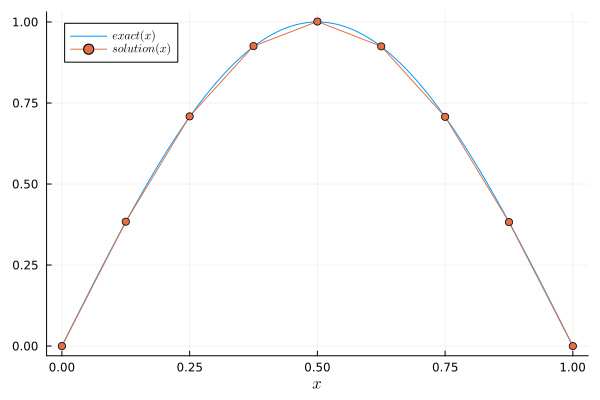
\includegraphics[width=0.5\textwidth]{images/solucao_aprox}

(TODO)

\paragraph{Convergência do Erro para Exemplo 1}
% 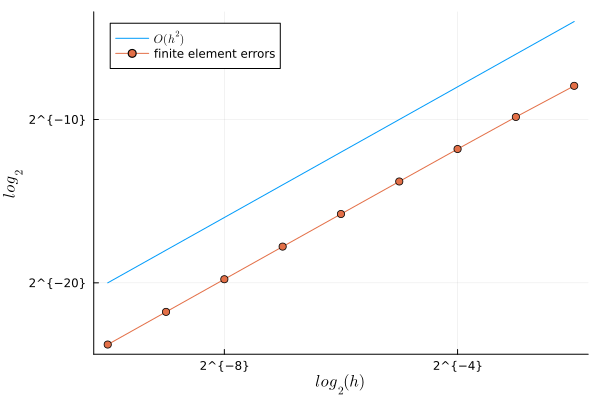
\includegraphics[width=0.5\textwidth]{images/convergencia_erro}

(TODO)

\paragraph{Solução Aproximada para Exemplo 2}

(TODO)

\end{document}
